%\VignetteEngine{knitr::knitr}
%\VignetteIndexEntry{Behavioral Change Point Analysis}

\documentclass[10pt]{article}\usepackage[]{graphicx}\usepackage[]{color}
%% maxwidth is the original width if it is less than linewidth
%% otherwise use linewidth (to make sure the graphics do not exceed the margin)
\makeatletter
\def\maxwidth{ %
  \ifdim\Gin@nat@width>\linewidth
    \linewidth
  \else
    \Gin@nat@width
  \fi
}
\makeatother

\definecolor{fgcolor}{rgb}{0.345, 0.345, 0.345}
\newcommand{\hlnum}[1]{\textcolor[rgb]{0.686,0.059,0.569}{#1}}%
\newcommand{\hlstr}[1]{\textcolor[rgb]{0.192,0.494,0.8}{#1}}%
\newcommand{\hlcom}[1]{\textcolor[rgb]{0.678,0.584,0.686}{\textit{#1}}}%
\newcommand{\hlopt}[1]{\textcolor[rgb]{0,0,0}{#1}}%
\newcommand{\hlstd}[1]{\textcolor[rgb]{0.345,0.345,0.345}{#1}}%
\newcommand{\hlkwa}[1]{\textcolor[rgb]{0.161,0.373,0.58}{\textbf{#1}}}%
\newcommand{\hlkwb}[1]{\textcolor[rgb]{0.69,0.353,0.396}{#1}}%
\newcommand{\hlkwc}[1]{\textcolor[rgb]{0.333,0.667,0.333}{#1}}%
\newcommand{\hlkwd}[1]{\textcolor[rgb]{0.737,0.353,0.396}{\textbf{#1}}}%

\usepackage{framed}
\makeatletter
\newenvironment{kframe}{%
 \def\at@end@of@kframe{}%
 \ifinner\ifhmode%
  \def\at@end@of@kframe{\end{minipage}}%
  \begin{minipage}{\columnwidth}%
 \fi\fi%
 \def\FrameCommand##1{\hskip\@totalleftmargin \hskip-\fboxsep
 \colorbox{shadecolor}{##1}\hskip-\fboxsep
     % There is no \\@totalrightmargin, so:
     \hskip-\linewidth \hskip-\@totalleftmargin \hskip\columnwidth}%
 \MakeFramed {\advance\hsize-\width
   \@totalleftmargin\z@ \linewidth\hsize
   \@setminipage}}%
 {\par\unskip\endMakeFramed%
 \at@end@of@kframe}
\makeatother

\definecolor{shadecolor}{rgb}{.97, .97, .97}
\definecolor{messagecolor}{rgb}{0, 0, 0}
\definecolor{warningcolor}{rgb}{1, 0, 1}
\definecolor{errorcolor}{rgb}{1, 0, 0}
\newenvironment{knitrout}{}{} % an empty environment to be redefined in TeX

\usepackage{alltt}
\usepackage{amsmath}
\usepackage{amstext}
\usepackage{graphicx}
\usepackage{color}        
\usepackage{multirow}
\usepackage{setspace}
\setlength{\parindent}{0in}
\setlength{\parskip}{\baselineskip}

\usepackage[colorlinks=true,urlcolor=blue]{hyperref}

\newcommand{\bc}{\begin{center}}
\newcommand{\ec}{\end{center}}

\newcommand{\ben}{\begin{enumerate}}
\newcommand{\een}{\end{enumerate}}
\newcommand{\I}{\item}

\newcommand{\beq}{\begin{eqnarray}}
\newcommand{\eeq}{\end{eqnarray}}
\newcommand{\ed}{\end{document}}

\usepackage[left=1in,top=1.25in,right=1in,bottom=1.25in]{geometry}
\usepackage{setspace}

\title{Behavioral Change Point Analysis in R:\\
The {\tt bcpa} package}

\author{Eliezer Gurarie,\\
Department of Statistics\\
School of Environmental and Forest Sciences\\
University of Washington, Seattle\\
\url{eliezg@u.washington.edu}}
\date{October 2013}
\IfFileExists{upquote.sty}{\usepackage{upquote}}{}

\begin{document}

\maketitle
\begin{spacing}{0.1}
\tableofcontents
\end{spacing}
\section{Background}

The \texttt{bcpa} package is designed to streamline the implementation of the ``behavioral change point analysis'' (BCPA, Gurarie et al.~2009) for any time-stamped movement data, i.e.~in which there are $X$, $Y$ and $T$ coordinates representing spatial locations and time of observation. 

The BCPA was developed in order to identify changes in animal behaviors that were obscured by visual inspection or standard techniques. Specific difficulties associated with movement data include the multi-dimensionality, auto- and cross-correlation, considerable internal structure (reflecting behavioral complexity), and data collection that can be error-ridden or be irregularly sampled.  The irregular sampling is a particulaly vexing problem for marine organism data, for which locations are usually transmitted only when the animal is at the surface, while most standard approaches to modeling movement (e.g.~the Correlated Random Walk) are only meaningful for regularly sampled data. 

The paper had attracted considerable interest from biologists and ecologists that collect animal movement data and are eager to identify structure in the behaviors.  Unfortunately, the code that was originally posted as supplementary material was incomplete and poorly documented, making the method somewhat inaccesible to practitioners without strong statistical or programming backgrounds.  After responding to (about) the hundredth email to share the code and offer some suggestions, and in light of a bevy of improvements to the code itelf (e.g.~greater speed by dropping some routines into C++, greater flexibility in visualizing and presenting the results, more usable ``tuning knobs'' and flexible syntax) it became clear that bundling the implementation in an R package would be the most efficient and tidy way to make it more accessible.  

  
\section{Summary of method}

The BCPA uses a likelihood-based method for identifying significant changes in movement parameter values across long, complex datasets by sweeping an analysis window over the timeseries and identifying the most likely changepoints, while simultaneously testing which, if any, of the parameters might have changed at that changepoint.  

Implementing the BCPA involves the following steps:

\ben
\I Pick a response time-series variable $X$.  One fairly robust variable is the persistence velocity $V_p = V \cos(\theta)$ where $V$ is speed = displacement/time interval and $\theta$ is turning angle.  Another alternative is simply $V$. 

\I Assume that the observations $X(t)$ are a observations from a stationary continuous-time Gaussian process with mean $\mu_i$, standard deviation $\sigma_i$ and time-scale of autocorrelation $\tau_i$, where $i \in (1,2,...N)$ represents an \emph{a priori} unknown number of behavioral states. \emph{Note: the use of a continuous time scale $\tau >0$ is a change from the original model, which estimates a discrete autocorrelation $0 < \rho < 1$.  The time-scale is more biologically meaningful, as it is estimated in units of time: the longer the time-scale the longer the ``memory'' of the movement}.

\I Obtain a likelihood for $\mu_i$, $\sigma_i$ and $\rho_i$ within a given stationary state $i$ (See Gurarie et al.~2009 for details).

\I Find the location within a window of observations which splits a subset of the data into two sets of the three parameters. 

\I Within this window, use a version of BIC to determine which combination (if any) of the three parameters most parsimoniously describes the separation in the data.  Often, the null model is returned.  I say "modified" because the BIC is usually defined as: $BIC = - 2 \log(L) + k \log(n)$, where $L$ is the likelihood, $k$ is the number of parameters, and $n$ is the number of data points; however, the 2 is replace with a constant $K > 0$.  The smaller this value, the more conservative the analysis, i.e.~the more likely it is to select a simpler or null model.  This is one of several ``tuning knobs'' in the BCPA. 

\I Sweep a window of fixed size across the time series and collect all the changepoints, the  associated models, and the values of the estimated parameters according to the selected model on either side of the changepoint within the window.   Note, the window size is another "knob" - larger windows are more robust but more coarse, smaller windows are more sensitive but more likely to give slightly spurious results, compensated by adjusting the $K$.
\een

These steps summarize the actual analysis.  The output of the analysis can be summarized and presented in two ways: 
 
\ben
\I Smooth BCPA: A ``smooth'' output is the one described in the original paper: is the average over all the estimated parameters, and the location of all the change points on the other.  This gives interesting output - with, in particular, the opportunity to have parameters change both suddenly and gradually, and to visualize a phase plot of the behavioral shifts - both sudden and gradual. 

\I Flat BCPA: A "flat" output takes the result of the window sweep and finds the most frequently chosen change points, clustering those unique changepoints which are close to each other (within some interval $dT_c$).  The three parameters $\mu$, $\sigma$ and $\tau$ are then estimated within each section, and the location of these ``flat'' changepoints is recorded.  This output is directly comparable to the BPMM segmentation. 
\een

\section{Detailed implementation}

The complete analysis can now be performed in, essentially, two or three lines of code (see final sections of this vignette).   Before leaping into them, I review the assumptions and fundamental pieces of the method, using the functions within \texttt{bcpa} to facilitate implementation.

\subsection{Estimating auto-correlation / characteristic time-scale for irregular data}

The BCPA (as currently implemented) analyzes a one-dimensional, arbitrarily sampled autocorrelated Gaussian time-series $X(t)$, specified by three parameters, a mean $\mu$, a standard deviation $\sigma$ and a characteristic time-scale $\tau$ (or autocorrelation coefficient $\rho$), such that:
\begin{eqnarray*}
  \text{E}{X(t)} &=& \mu	\nonumber\\
	\text{Var}{X(t)} &=& \sigma^2 \nonumber\\
	\text{Cor}{X(t)}{X(t-\Delta t)} &=& \exp(-\Delta t/\tau) = \rho^{\Delta t},
\end{eqnarray*}
\noindent 
The characteristic time-scale is an innovation over the original implementation, which estimated $\rho$.  The interpretation of  $\rho$, which ranges from 0 to 1, depends on the units of the time measurement - and can flirt with being uninformatively close to 0 or 1, whereas the time scale is a measurement of the temporal range of correlation in the movement, with somewhat more intuitive biological interpretation (Gurarie and Ovaskainen 2011).

These relationships are used to obtain a likelihood for observations $X_i$ observed at times $T_i$, and the likelihood is maximized to estimate the characteristic time scale. In the \texttt{bcpa} package, this is done with the \texttt{GetRho} function, which is driven by the \texttt{GetL} function (encoded in C++).  Examples are given below:

Loading the package
\begin{knitrout}
\definecolor{shadecolor}{rgb}{0.969, 0.969, 0.969}\color{fgcolor}\begin{kframe}
\begin{alltt}
\hlkwd{library}\hlstd{(bcpa)}
\end{alltt}
\end{kframe}
\end{knitrout}


Simulating a gappy, Gaussian, time series

\begin{knitrout}
\definecolor{shadecolor}{rgb}{0.969, 0.969, 0.969}\color{fgcolor}\begin{kframe}
\begin{alltt}
\hlstd{rho} \hlkwb{<-} \hlnum{0.8}
\hlstd{x.full} \hlkwb{<-} \hlkwd{arima.sim}\hlstd{(}\hlnum{1000}\hlstd{,} \hlkwc{model} \hlstd{=} \hlkwd{list}\hlstd{(}\hlkwc{ar} \hlstd{= rho))}
\hlstd{t.full} \hlkwb{<-} \hlnum{1}\hlopt{:}\hlnum{1000}
\hlstd{keep} \hlkwb{<-} \hlkwd{sort}\hlstd{(}\hlkwd{sample}\hlstd{(}\hlnum{1}\hlopt{:}\hlnum{1000}\hlstd{,} \hlnum{200}\hlstd{))}
\hlstd{x} \hlkwb{<-} \hlstd{x.full[keep]}
\hlstd{t} \hlkwb{<-} \hlstd{t.full[keep]}
\hlkwd{plot}\hlstd{(t, x,} \hlkwc{type} \hlstd{=} \hlstr{"l"}\hlstd{)}
\end{alltt}
\end{kframe}
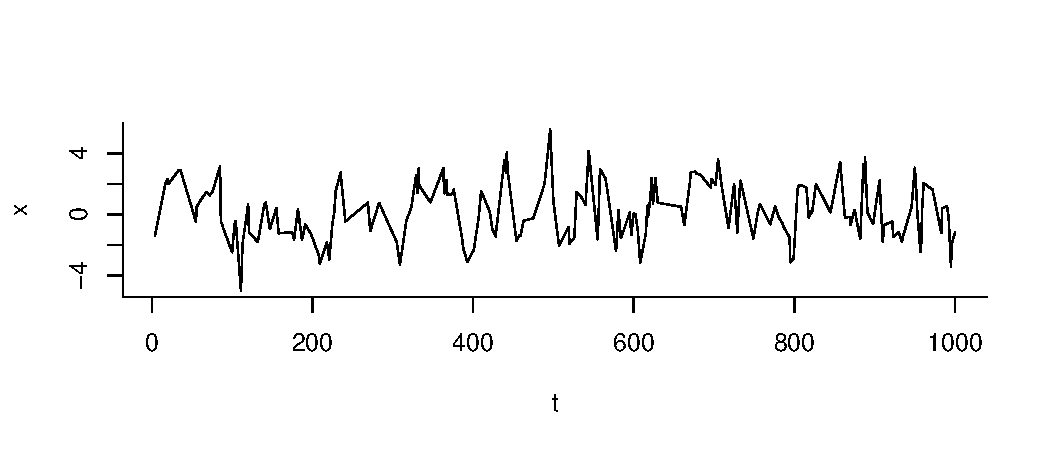
\includegraphics[width=\textwidth]{figure/GetRhoDemo1} 

\end{knitrout}


Obtaining the likelihood function for different values of $\rho$.

\begin{knitrout}
\definecolor{shadecolor}{rgb}{0.969, 0.969, 0.969}\color{fgcolor}\begin{kframe}
\begin{alltt}
\hlstd{rhos} \hlkwb{<-} \hlkwd{seq}\hlstd{(}\hlnum{0}\hlstd{,}\hlnum{.99}\hlstd{,}\hlnum{.01}\hlstd{)}
\hlstd{L} \hlkwb{<-} \hlkwd{rep}\hlstd{(}\hlnum{NA}\hlstd{,} \hlkwd{length}\hlstd{(rhos))}
\hlkwa{for}\hlstd{(i} \hlkwa{in} \hlnum{1}\hlopt{:}\hlkwd{length}\hlstd{(rhos))}
  \hlstd{L[i]} \hlkwb{<-} \hlkwd{GetL}\hlstd{(x,t,rhos[i])}
\hlcom{# plot likelihood profile}
\hlkwd{plot}\hlstd{(rhos, L,} \hlkwc{type}\hlstd{=}\hlstr{"l"}\hlstd{)}
\hlkwd{abline}\hlstd{(}\hlkwc{v} \hlstd{= rho,} \hlkwc{lty}\hlstd{=}\hlnum{2}\hlstd{,} \hlkwc{lwd}\hlstd{=}\hlnum{2}\hlstd{);} \hlkwd{abline}\hlstd{(}\hlkwc{v} \hlstd{= rhos[L} \hlopt{==} \hlkwd{max}\hlstd{(L)],} \hlkwc{lty}\hlstd{=}\hlnum{3}\hlstd{,} \hlkwc{lwd}\hlstd{=}\hlnum{2}\hlstd{)}
\hlkwd{legend}\hlstd{(}\hlstr{"bottomleft"}\hlstd{,} \hlkwc{legend}\hlstd{=}\hlkwd{c}\hlstd{(}\hlstr{"true value"}\hlstd{,}\hlstr{"MLE"}\hlstd{),} \hlkwc{lty}\hlstd{=}\hlnum{2}\hlopt{:}\hlnum{3}\hlstd{,} \hlkwc{lwd}\hlstd{=}\hlnum{2}\hlstd{)}
\end{alltt}
\end{kframe}
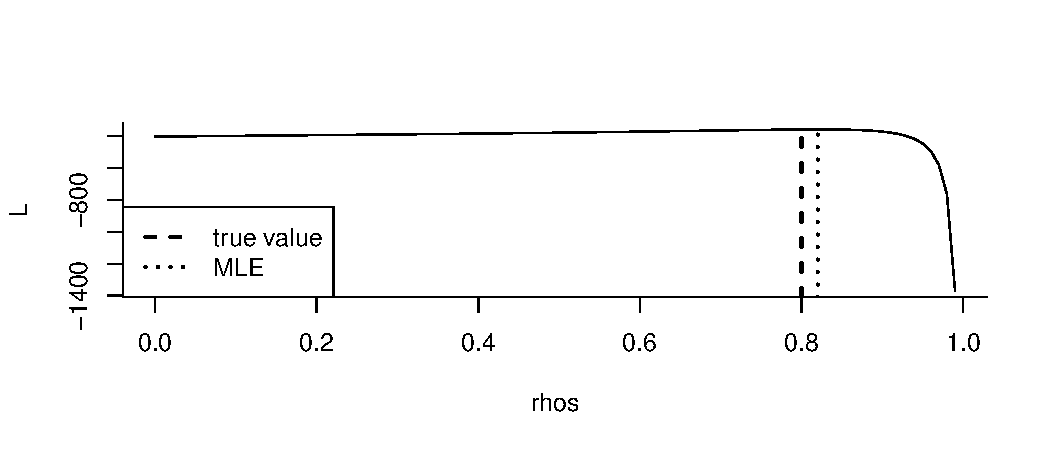
\includegraphics[width=\textwidth]{figure/GetRhoDemo2} 

\end{knitrout}


Using the \texttt{GetRho} function to estimate $\rho$ or $\tau$:
\begin{knitrout}
\definecolor{shadecolor}{rgb}{0.969, 0.969, 0.969}\color{fgcolor}\begin{kframe}
\begin{alltt}
\hlkwd{GetRho}\hlstd{(x, t,} \hlkwc{tau} \hlstd{=} \hlnum{FALSE}\hlstd{)}
\end{alltt}
\begin{verbatim}
##   rho.hat        LL 
##    0.8209 -357.6468
\end{verbatim}
\begin{alltt}
\hlkwd{GetRho}\hlstd{(x, t,} \hlkwc{tau} \hlstd{=} \hlnum{TRUE}\hlstd{)}
\end{alltt}
\begin{verbatim}
##  rho.hat       LL 
##    5.067 -357.647
\end{verbatim}
\end{kframe}
\end{knitrout}

{\bf Future work:  It is straightforward to obtain confidence intervals around this estimate.}

\subsection{Speeds and turning angles}

To apply the method to movement data of the form ${\bf Z}_i,T_i$, where ${\bf Z}_i$ represents the location vector at time $T_i$, it is necessary to extract a one-dimensional time series that conforms to the assumption.  Examples which generally conforms to the assumptions are the ``persistence'' velocity velocity $V_p(t)$ and turning velocity $V_t(t)$:

  \begin{eqnarray}
  	V_p(T_i) = V(T_i) \cos(\Theta(T_i))\\
		V_t(T_i) = V(T_i) \sin(\Theta(T_i))
	\end{eqnarray}

where $V(T_i) = ||{\bf Z}_i - {\bf Z}_{i-1}||/(T_i - T_{i-1})$ is the scalar speed at time $T_i$.  $V_p$ captures the tendency and magnitude of a movement to persist in a given direction while $V_t$ captures the tendency of movement to head in a perpendicular direction in a given time interval.  Thus, the primary descriptive features of movement, namely speed, directional persistence, and variability are captured in these variables.  Alternatively, the log of step lengths can have a roughly Gaussian distribution.

For demonstration purposes, we include a simulated movement data set called \texttt{Simp}:
\bc
\begin{knitrout}
\definecolor{shadecolor}{rgb}{0.969, 0.969, 0.969}\color{fgcolor}\begin{kframe}
\begin{alltt}
\hlkwd{data}\hlstd{(Simp)}
\hlkwd{head}\hlstd{(Simp)}
\end{alltt}
\begin{verbatim}
##   Time     X       Y
## 1 0.18 23.75  -9.064
## 2 0.22 26.75 -11.325
## 3 0.74 13.25   2.946
## 4 0.88 28.46  26.634
## 5 1.40 96.78 121.783
## 6 1.41 97.86 123.348
\end{verbatim}
\begin{alltt}
\hlkwd{plot}\hlstd{(Simp)}
\end{alltt}
\end{kframe}
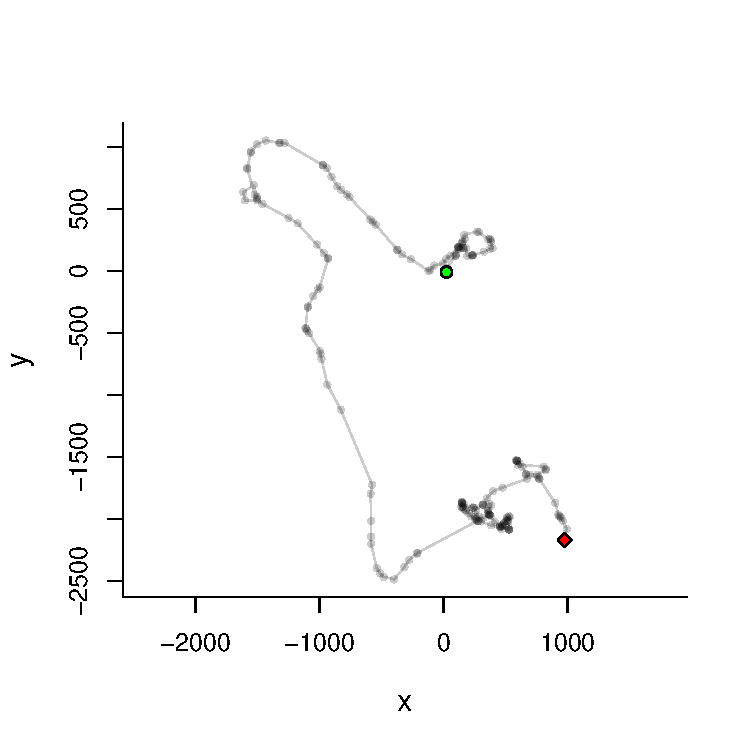
\includegraphics[width=0.7\textwidth]{figure/Simp} 

\end{knitrout}

\ec
The \texttt{Simp} objects is of class ``track'', which is simply a data frame with columns $X$, $Y$ and $T$, and the \texttt{bcpa} package contains a plotting method for  a track of this form with a green circle illustrating the start and a red rhombus indicating the end of the track.

To obtain the step length and turning angles, use the \texttt{GetVT} function, which decomposes the data into single step and all the relevant statistics:
\begin{knitrout}
\definecolor{shadecolor}{rgb}{0.969, 0.969, 0.969}\color{fgcolor}\begin{kframe}
\begin{alltt}
\hlstd{Simp.VT} \hlkwb{<-} \hlkwd{GetVT}\hlstd{(Simp)}
\hlkwd{head}\hlstd{(Simp.VT)}
\end{alltt}
\begin{verbatim}
##          Z.start          Z.end      S    Phi    Theta T.start T.end T.mid
## 2  26.75- 11.33i  13.25+  2.95i  19.64 2.3282  2.97445    0.22  0.74 0.480
## 3  13.25+  2.95i  28.46+ 26.63i  28.15 1.0000 -1.32815    0.74  0.88 0.810
## 4  28.46+ 26.63i  96.78+121.78i 117.13 0.9481 -0.05195    0.88  1.40 1.140
## 5  96.78+121.78i  97.86+123.35i   1.90 0.9674  0.01930    1.40  1.41 1.405
## 6  97.86+123.35i 101.47+135.40i  12.59 1.2797  0.31228    1.41  1.48 1.445
## 7 101.47+135.40i 117.74+193.35i  60.19 1.2971  0.01739    1.48  2.00 1.740
##     dT      V T.POSIX
## 2 0.52  37.77   0.480
## 3 0.14 201.08   0.810
## 4 0.52 225.26   1.140
## 5 0.01 189.97   1.405
## 6 0.07 179.80   1.445
## 7 0.52 115.75   1.740
\end{verbatim}
\end{kframe}
\end{knitrout}

The overall persistence of the movement and distribution of step lengths:
\bc
\begin{knitrout}
\definecolor{shadecolor}{rgb}{0.969, 0.969, 0.969}\color{fgcolor}\begin{kframe}
\begin{alltt}
\hlkwd{par}\hlstd{(}\hlkwc{mfrow} \hlstd{=} \hlkwd{c}\hlstd{(}\hlnum{1}\hlstd{,} \hlnum{2}\hlstd{))}
\hlkwd{hist}\hlstd{(Simp.VT}\hlopt{$}\hlstd{V,} \hlkwc{breaks} \hlstd{=} \hlnum{20}\hlstd{,} \hlkwc{col} \hlstd{=} \hlstr{"grey"}\hlstd{)}
\hlkwd{hist}\hlstd{(Simp.VT}\hlopt{$}\hlstd{Theta,} \hlkwc{breaks} \hlstd{=} \hlnum{20}\hlstd{,} \hlkwc{col} \hlstd{=} \hlstr{"grey"}\hlstd{)}
\end{alltt}
\end{kframe}
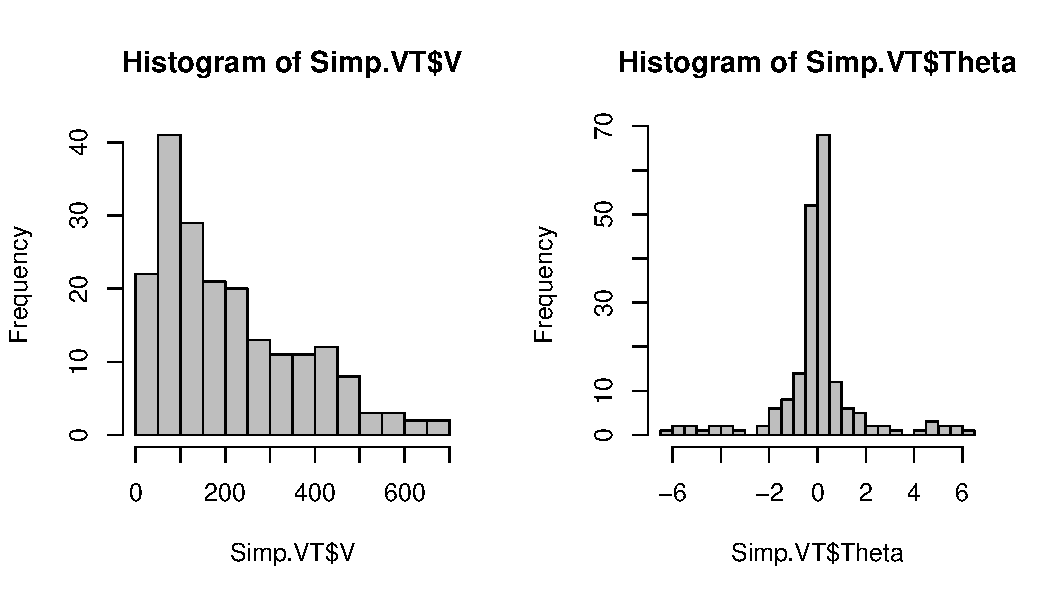
\includegraphics[width=0.8\textwidth]{figure/Histograms} 

\end{knitrout}

\ec


\subsection{Obtaining a changepoint}

A single changepoint in a time-series where the parameters change at some unknown timepoints $t^*$ is done by simply sweeping all possible breaks, and finding the most-likely changepoint according to the likelihood.  This is illustrated below:

\begin{knitrout}
\definecolor{shadecolor}{rgb}{0.969, 0.969, 0.969}\color{fgcolor}\begin{kframe}
\begin{alltt}
\hlkwd{par}\hlstd{(}\hlkwc{bty}\hlstd{=}\hlstr{"l"}\hlstd{)}
\hlstd{mu1} \hlkwb{<-} \hlnum{5}\hlstd{; mu2} \hlkwb{<-} \hlnum{3}
\hlstd{sigma1} \hlkwb{<-} \hlnum{2}\hlstd{; sigma2} \hlkwb{<-} \hlnum{1}
\hlstd{rho1} \hlkwb{<-} \hlnum{0.5}\hlstd{; rho2} \hlkwb{<-} \hlnum{0.5}

\hlstd{SimTS} \hlkwb{<-} \hlkwa{function}\hlstd{(}\hlkwc{n}\hlstd{,} \hlkwc{mu}\hlstd{,} \hlkwc{rho}\hlstd{,} \hlkwc{sigma}\hlstd{)}
\hlstd{\{}
  \hlstd{X.standard} \hlkwb{<-} \hlkwd{arima.sim}\hlstd{(n,} \hlkwc{model}\hlstd{=}\hlkwd{list}\hlstd{(}\hlkwc{ar} \hlstd{= rho))}
  \hlstd{X.standard}\hlopt{/}\hlkwd{sd}\hlstd{(X.standard)}\hlopt{*}\hlstd{sigma} \hlopt{+} \hlstd{mu}
\hlstd{\}}

\hlcom{# create time series with break at 500}
\hlstd{t.full} \hlkwb{<-} \hlnum{1}\hlopt{:}\hlnum{1000}
\hlstd{t.break} \hlkwb{<-} \hlnum{500}
\hlstd{x.full} \hlkwb{<-} \hlkwd{c}\hlstd{(}\hlkwd{SimTS}\hlstd{(t.break, mu1, rho1, sigma1),}
            \hlkwd{SimTS}\hlstd{(}\hlkwd{max}\hlstd{(t.full)}\hlopt{-}\hlstd{t.break}\hlopt{+}\hlnum{1}\hlstd{, mu2, rho2, sigma2))}

\hlcom{# subsample 100 observations and estimate}
\hlstd{keep} \hlkwb{<-} \hlkwd{sort}\hlstd{(}\hlkwd{sample}\hlstd{(}\hlnum{1}\hlopt{:}\hlkwd{length}\hlstd{(x.full),} \hlnum{100}\hlstd{))}
\hlstd{x} \hlkwb{<-} \hlstd{x.full[keep]}
\hlstd{t} \hlkwb{<-} \hlstd{t.full[keep]}
\hlstd{(BB} \hlkwb{<-} \hlkwd{GetBestBreak}\hlstd{(x,t,} \hlkwc{tau}\hlstd{=}\hlnum{FALSE}\hlstd{))}
\end{alltt}
\begin{verbatim}
##    bb.index     bb.time         mu1          s1     rho.hat          LL 
##     51.0000    482.0000      5.1092      2.0183      0.5548   -104.1158 
##         mu2          s2     rho.hat          LL ll.total.LL 
##      3.0158      0.9065      0.7785    -58.0164   -162.1321
\end{verbatim}
\end{kframe}
\end{knitrout}


The estimates should be fairly good (note that we are chosing to estimate $\rho$ rather than $\tau$).
\bc
\begin{knitrout}
\definecolor{shadecolor}{rgb}{0.969, 0.969, 0.969}\color{fgcolor}\begin{kframe}
\begin{alltt}
\hlkwd{plot}\hlstd{(t,x,} \hlkwc{type}\hlstd{=}\hlstr{"l"}\hlstd{)}
\hlkwd{abline}\hlstd{(}\hlkwc{v} \hlstd{=} \hlnum{500}\hlstd{,} \hlkwc{col}\hlstd{=}\hlnum{2}\hlstd{,} \hlkwc{lwd}\hlstd{=}\hlnum{2}\hlstd{,} \hlkwc{lty}\hlstd{=}\hlnum{2}\hlstd{);} \hlkwd{abline}\hlstd{(}\hlkwc{v} \hlstd{= BB[}\hlnum{2}\hlstd{],} \hlkwc{col}\hlstd{=}\hlnum{2}\hlstd{,} \hlkwc{lwd}\hlstd{=}\hlnum{2}\hlstd{,} \hlkwc{lty}\hlstd{=}\hlnum{3}\hlstd{)}
\hlkwd{legend}\hlstd{(}\hlstr{"topright"}\hlstd{,} \hlkwc{legend}\hlstd{=}\hlkwd{c}\hlstd{(}\hlstr{"true break"}\hlstd{,} \hlstr{"estimated break"}\hlstd{),} \hlkwc{col}\hlstd{=}\hlnum{2}\hlstd{,} \hlkwc{lwd}\hlstd{=}\hlnum{2}\hlstd{,} \hlkwc{lty}\hlstd{=}\hlnum{2}\hlopt{:}\hlnum{3}\hlstd{)}
\end{alltt}
\end{kframe}
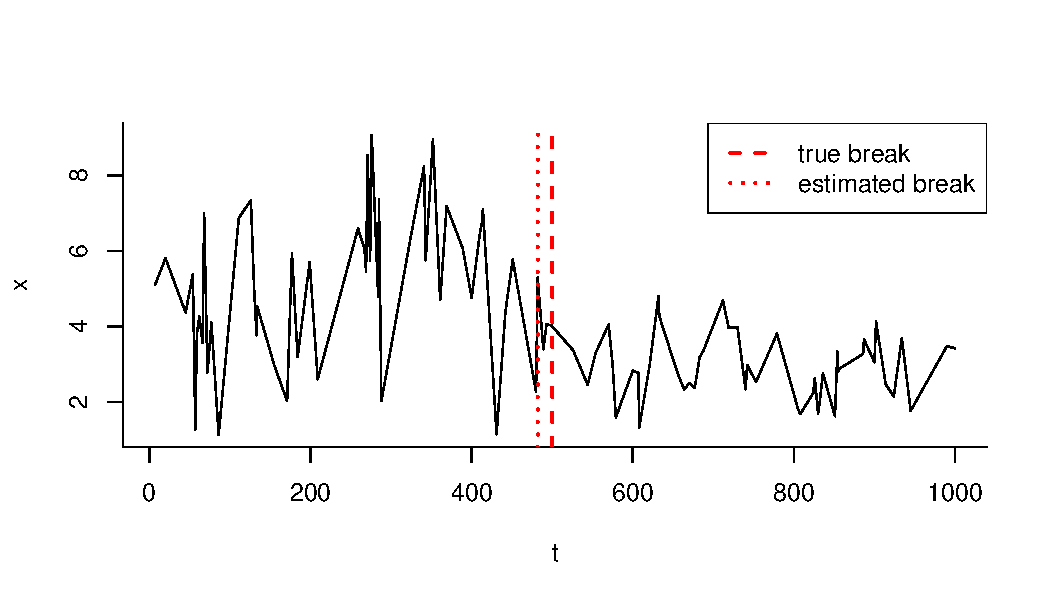
\includegraphics[width=0.8\textwidth]{figure/OneBreak2} 

\end{knitrout}

\ec

The likelihood is used to obtain a BIC value for all of the possible models.  The possible models are numbered M0 to M7, corresponding to no significant changes (M0), only $\mu$, $\sigma$ or $\rho$ changing (M1, M2, M3, respectively), both of $\mu$ and $\sigma$, $\mu$ and $\rho$ and $\sigma$ and $\rho$ changing (M4, M5, M6), and all three parameters changing (M7).  The model are compared with the \texttt{GetModels} function:

\begin{knitrout}
\definecolor{shadecolor}{rgb}{0.969, 0.969, 0.969}\color{fgcolor}\begin{kframe}
\begin{alltt}
\hlkwd{GetModels}\hlstd{(x, t, BB[}\hlnum{1}\hlstd{],} \hlkwc{tau} \hlstd{=} \hlnum{FALSE}\hlstd{)}
\end{alltt}
\begin{verbatim}
##      Model     LL   bic   mu1    s1   rho1   mu2     s2   rho2
## [1,]     0 -193.7 401.3 4.061 1.888 0.7661 4.061 1.8885 0.7661
## [2,]     1 -178.9 380.8 5.109 1.553 0.5540 2.969 1.5526 0.5540
## [3,]     2 -193.6 410.1 4.061 2.018 0.8683 4.061 0.8533 0.8683
## [4,]     3 -191.1 405.2 4.061 1.888 0.5548 4.061 1.8885 0.7533
## [5,]     4 -161.8 351.2 5.109 2.018 0.6433 2.969 0.8533 0.6433
## [6,]     5 -177.0 381.7 5.109 1.553 0.5548 2.969 1.5526 0.7533
## [7,]     6 -192.5 412.6 4.061 2.018 0.5548 4.061 0.8533 0.7533
## [8,]     7 -161.2 354.6 5.109 2.018 0.5548 2.969 0.8533 0.7533
\end{verbatim}
\end{kframe}
\end{knitrout}

The model selection should select model 4 ($\mu$ and $\sigma$ change) as having the lowest BIC.  

This is with the default sensitivity parameter $K=2$, which comes from the definition of the BIC $= -Kn \log(L) + k \log(n)$ (see summary in section 2).  If we lower this value, a simpler model is more likely to be selected:
\begin{knitrout}
\definecolor{shadecolor}{rgb}{0.969, 0.969, 0.969}\color{fgcolor}\begin{kframe}
\begin{alltt}
\hlkwd{GetModels}\hlstd{(x, t, BB[}\hlnum{1}\hlstd{],} \hlkwc{tau} \hlstd{=} \hlnum{FALSE}\hlstd{,} \hlkwc{K} \hlstd{=} \hlnum{0.5}\hlstd{)}
\end{alltt}
\begin{verbatim}
##      Model     LL   bic   mu1    s1   rho1   mu2     s2   rho2
## [1,]     0 -193.7 110.7 4.061 1.888 0.7661 4.061 1.8885 0.7661
## [2,]     1 -178.9 112.5 5.109 1.553 0.5540 2.969 1.5526 0.5540
## [3,]     2 -193.6 119.8 4.061 2.018 0.8683 4.061 0.8533 0.8683
## [4,]     3 -191.1 118.6 4.061 1.888 0.5548 4.061 1.8885 0.7533
## [5,]     4 -161.8 108.5 5.109 2.018 0.6433 2.969 0.8533 0.6433
## [6,]     5 -177.0 116.1 5.109 1.553 0.5548 2.969 1.5526 0.7533
## [7,]     6 -192.5 123.9 4.061 2.018 0.5548 4.061 0.8533 0.7533
## [8,]     7 -161.2 112.8 5.109 2.018 0.5548 2.969 0.8533 0.7533
\end{verbatim}
\end{kframe}
\end{knitrout}


And if we increase it, more complex models are likely to be selected
\begin{knitrout}
\definecolor{shadecolor}{rgb}{0.969, 0.969, 0.969}\color{fgcolor}\begin{kframe}
\begin{alltt}
\hlkwd{GetModels}\hlstd{(x, t, BB[}\hlnum{1}\hlstd{],} \hlkwc{tau} \hlstd{=} \hlnum{FALSE}\hlstd{,} \hlkwc{K} \hlstd{=} \hlnum{5}\hlstd{)}
\end{alltt}
\begin{verbatim}
##      Model     LL   bic   mu1    s1   rho1   mu2     s2   rho2
## [1,]     0 -193.7 982.4 4.061 1.888 0.7661 4.061 1.8885 0.7661
## [2,]     1 -178.9 917.4 5.109 1.553 0.5540 2.969 1.5526 0.5540
## [3,]     2 -193.6 990.8 4.061 2.018 0.8683 4.061 0.8533 0.8683
## [4,]     3 -191.1 978.5 4.061 1.888 0.5548 4.061 1.8885 0.7533
## [5,]     4 -161.8 836.5 5.109 2.018 0.6433 2.969 0.8533 0.6433
## [6,]     5 -177.0 912.7 5.109 1.553 0.5548 2.969 1.5526 0.7533
## [7,]     6 -192.5 990.1 4.061 2.018 0.5548 4.061 0.8533 0.7533
## [8,]     7 -161.2 838.2 5.109 2.018 0.5548 2.969 0.8533 0.7533
\end{verbatim}
\end{kframe}
\end{knitrout}


Below, we change only the autocorrelation parameter, which is quite a bit more difficult to detect by eye:
\bc
\begin{knitrout}
\definecolor{shadecolor}{rgb}{0.969, 0.969, 0.969}\color{fgcolor}\begin{kframe}
\begin{alltt}
\hlstd{mu1} \hlkwb{<-} \hlnum{0}
\hlstd{mu2} \hlkwb{<-} \hlnum{0}
\hlstd{sigma1} \hlkwb{<-} \hlnum{1}
\end{alltt}


{\ttfamily\noindent\color{warningcolor}{\#\# Warning: NA/Inf replaced by maximum positive value}}\end{kframe}
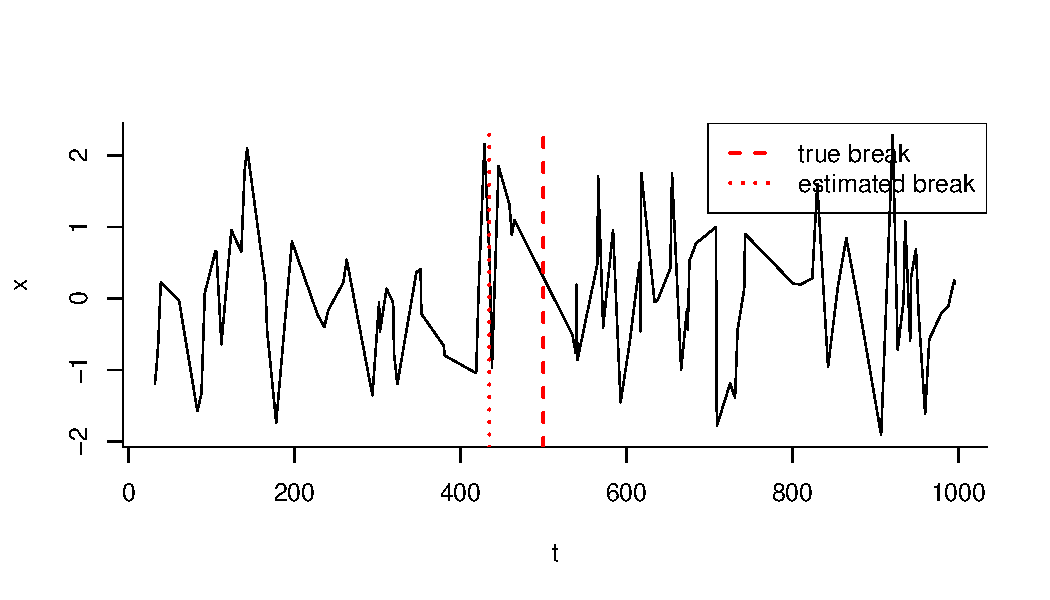
\includegraphics[width=0.8\textwidth]{figure/OneBreak3} 

\end{knitrout}

\ec
The model selection should select model 4 (only $\rho$ changes):

\begin{knitrout}
\definecolor{shadecolor}{rgb}{0.969, 0.969, 0.969}\color{fgcolor}\begin{kframe}
\begin{alltt}
\hlkwd{GetModels}\hlstd{(x, t, BB[}\hlnum{1}\hlstd{],} \hlkwc{tau} \hlstd{=} \hlnum{FALSE}\hlstd{)}
\end{alltt}
\begin{verbatim}
##      Model     LL   bic      mu1     s1   rho1    mu2     s2      rho2
## [1,]     0 -133.3 280.5  0.01470 0.9400 0.5022 0.0147 0.9400 0.5021875
## [2,]     1 -131.7 286.4 -0.07943 0.9364 0.4731 0.0857 0.9364 0.4730730
## [3,]     2 -131.3 285.6  0.01470 0.9061 0.5475 0.0147 0.9666 0.5474696
## [4,]     3 -122.1 267.2  0.01470 0.9400 0.8828 0.0147 0.9400 0.0005311
## [5,]     4 -131.2 289.9 -0.07943 0.9061 0.5308 0.0857 0.9666 0.5307844
## [6,]     5 -121.8 271.3 -0.07943 0.9364 0.8828 0.0857 0.9364 0.0005311
## [7,]     6 -122.0 271.6  0.01470 0.9061 0.8828 0.0147 0.9666 0.0005311
## [8,]     7 -121.7 275.7 -0.07943 0.9061 0.8828 0.0857 0.9666 0.0005311
\end{verbatim}
\end{kframe}
\end{knitrout}


\subsection{Applying the window sweep}

The main wrapper function for the complete analysis is \texttt{WindowSweep}.  We select a windowsize and sensitivity parameter $K$ and sweep analysis windows across the entire time series:

\begin{knitrout}
\definecolor{shadecolor}{rgb}{0.969, 0.969, 0.969}\color{fgcolor}\begin{kframe}
\begin{alltt}
\hlstd{Simp.ws} \hlkwb{<-} \hlkwd{WindowSweep}\hlstd{(Simp.VT,} \hlstr{"V*cos(Theta)"}\hlstd{,} \hlkwc{windowsize} \hlstd{=} \hlnum{50}\hlstd{,} \hlkwc{progress} \hlstd{=} \hlnum{FALSE}\hlstd{,}
    \hlkwc{K} \hlstd{=} \hlnum{2}\hlstd{)}
\end{alltt}
\end{kframe}
\end{knitrout}


Note that the second argument of the function is a character string within which any function of the columns of the VT table can be analyzed as a response. 

The key portion of the output of this function is the ``windowsweep'' data frame, which contains the proposed break (last column), the parameters to the left and right of the break, and the selected model:

\begin{knitrout}
\definecolor{shadecolor}{rgb}{0.969, 0.969, 0.969}\color{fgcolor}\begin{kframe}
\begin{alltt}
\hlkwd{head}\hlstd{(Simp.ws}\hlopt{$}\hlstd{ws)}
\end{alltt}
\begin{verbatim}
##   Model     LL   bic   mu1    s1   rho1   mu2    s2   rho2 Break.bb.time
## 1     1 -288.6 596.8 110.5 142.6 0.6908 348.4 142.6 0.6908         7.625
## 2     1 -288.3 596.2 112.3 145.3 0.7268 329.1 145.3 0.7268         7.405
## 3     1 -288.0 595.6 114.5 146.0 0.7487 323.4 146.0 0.7487         7.405
## 4     1 -289.8 599.2 111.7 142.9 0.5501 331.5 142.9 0.5501         7.565
## 5     1 -285.2 590.1 117.9 111.6 0.3901 427.4 111.6 0.3901        10.130
## 6     1 -285.3 590.2 116.4 111.3 0.3851 426.5 111.3 0.3851        10.130
\end{verbatim}
\end{kframe}
\end{knitrout}


Note that in this example, the first 4 windows detect no changes in the  parameter values (Model 0) so the values are the same to the left and to the right of each changepoint. (A minor note: the \texttt{rho1} and \texttt{rho2} columns correspond to $\tau_1$ and $\tau_2$ - i.e.~the time-scales.)  

The following functions plot the output of the ``smooth'' summary, i.e.~the summary in which all the windows are averaged to obtain the ``smooth'' model.  In these plots, the vertical lines represent the significant change points, the width of the lines is proportional to the number of time that change point was selected, the black an dred lines represent the mean and standard deviation estimate, and the colors reflect the autocorrelation time-scale (bluer colors have smaller autocorrelation time scales).

\begin{knitrout}\small
\definecolor{shadecolor}{rgb}{0.969, 0.969, 0.969}\color{fgcolor}\begin{kframe}
\begin{alltt}
\hlkwd{plot}\hlstd{(Simp.ws,} \hlkwc{type} \hlstd{=} \hlstr{"smooth"}\hlstd{)}
\hlkwd{plot}\hlstd{(Simp.ws,} \hlkwc{type} \hlstd{=} \hlstr{"smooth"}\hlstd{,} \hlkwc{threshold} \hlstd{=} \hlnum{7}\hlstd{)}
\end{alltt}
\end{kframe}
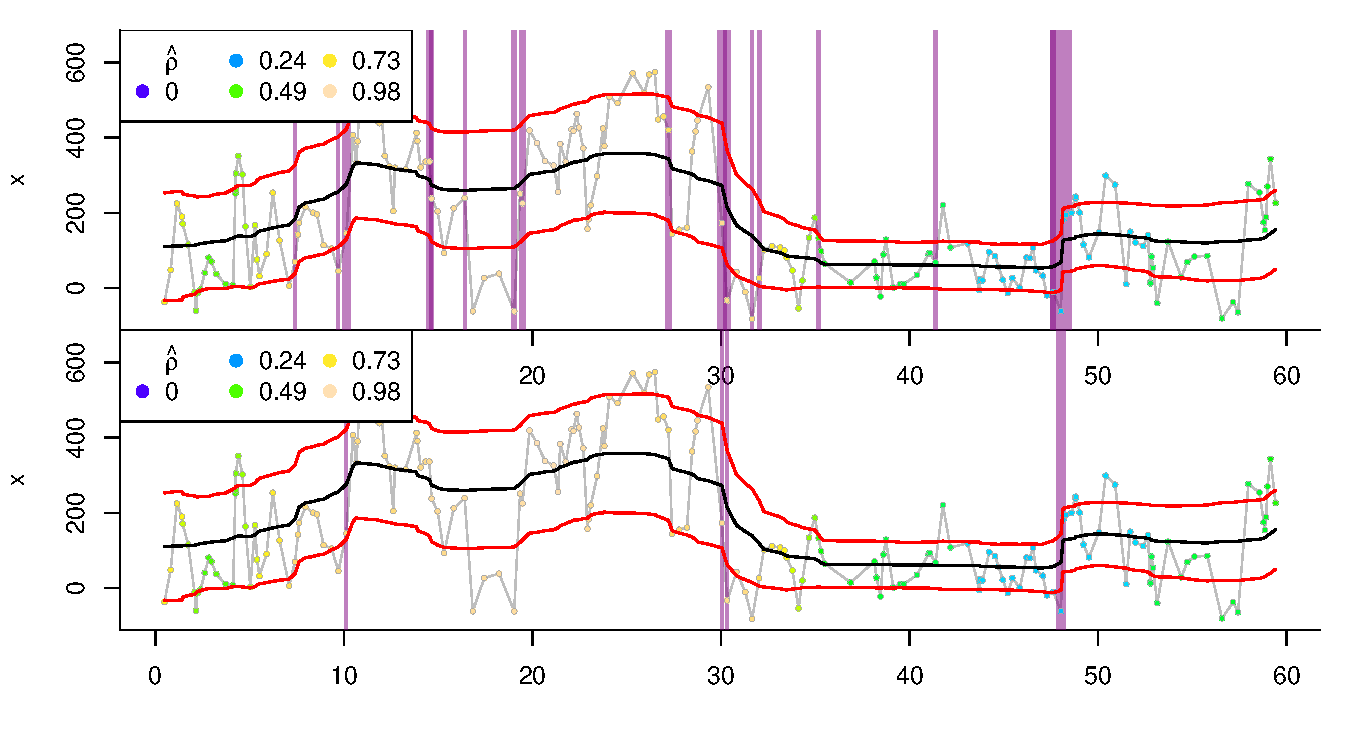
\includegraphics[width=\textwidth]{figure/BCPAsmooth} 

\end{knitrout}



The \texttt{threshold} parameter indicates how many of the windows that were swept over the data must have selected that changepoint for it to be considered significant.  The changepoints selected (at that threshold) are almost exactly the ones that were encoded in the original simulaiton. 

The ``flat'' analysis first selects changepoints that it deeps significant by clustering neighboring changepoints, and then estimates a homogeneous behavior between those changepoints.  Note that by increasing the clusterwisth to 3, many of the more minor changepoints are filtered away and the resulting profile is fairly uniform.

\begin{knitrout}\small
\definecolor{shadecolor}{rgb}{0.969, 0.969, 0.969}\color{fgcolor}\begin{kframe}
\begin{alltt}
\hlkwd{plot}\hlstd{(Simp.ws,} \hlkwc{type} \hlstd{=} \hlstr{"flat"}\hlstd{)}
\hlkwd{plot}\hlstd{(Simp.ws,} \hlkwc{type} \hlstd{=} \hlstr{"flat"}\hlstd{,} \hlkwc{clusterwidth} \hlstd{=} \hlnum{3}\hlstd{)}
\end{alltt}
\end{kframe}
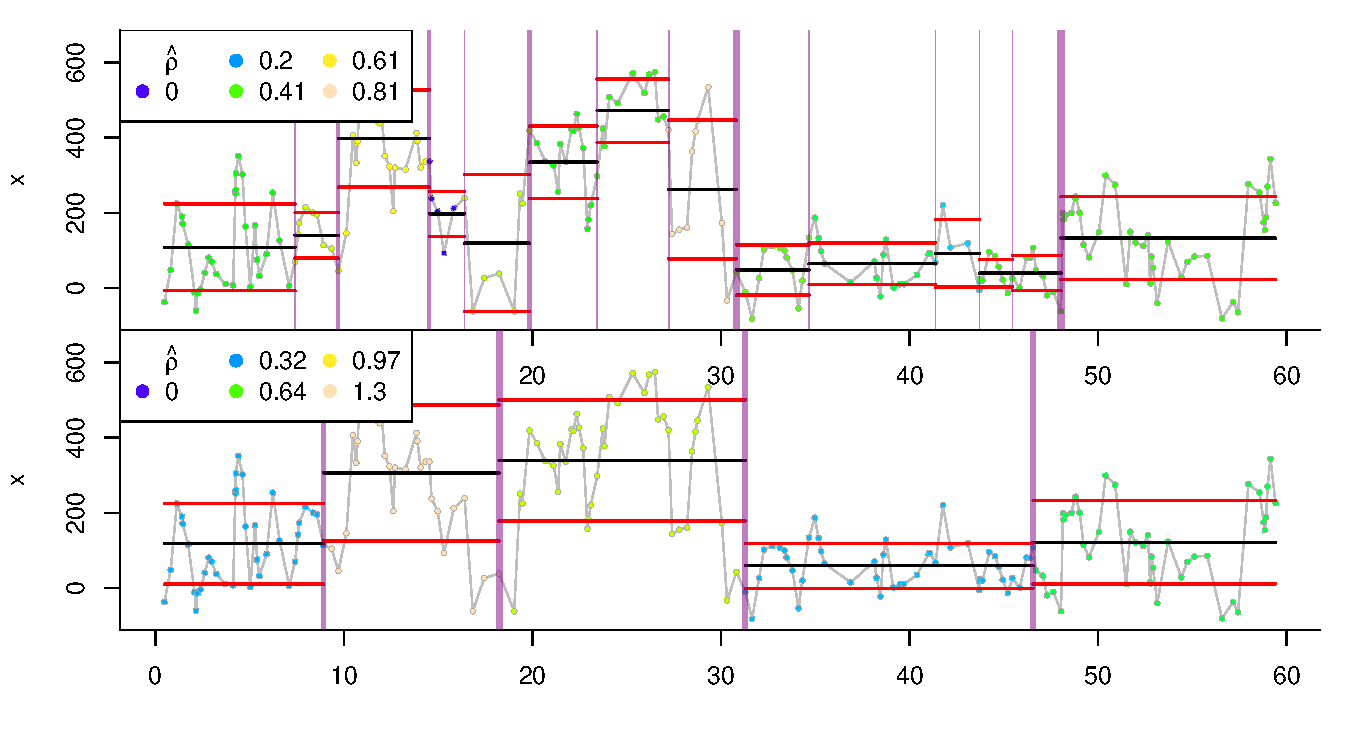
\includegraphics[width=\textwidth]{figure/BCPAflat} 

\end{knitrout}


A summary of the flat changepoints can be obtained as follows: 
\begin{knitrout}
\definecolor{shadecolor}{rgb}{0.969, 0.969, 0.969}\color{fgcolor}\begin{kframe}
\begin{alltt}
\hlkwd{ChangePointSummary}\hlstd{(Simp.ws,} \hlkwc{clusterwidth} \hlstd{=} \hlnum{3}\hlstd{)}
\end{alltt}
\begin{verbatim}
## $breaks
##   middle size modelmode middle.POSIX
## 1  8.972   23         1        9.133
## 2 18.609   45         1       18.630
## 3 31.082   39         4       31.053
## 4 46.605   40         1       46.630
## 
## $phases
##          t.cut mu.hat s.hat rho.hat     t0     t1 interval
## 1 (-0.52,8.97] 118.24 107.7  0.3511 -0.520  8.972    9.492
## 2  (8.97,18.6] 306.38 180.6  1.2868  8.972 18.609    9.637
## 3  (18.6,31.1] 339.79 161.0  0.8083 18.609 31.082   12.473
## 4  (31.1,46.6]  59.51  59.9  0.3678 31.082 46.605   15.523
## 5  (46.6,59.4] 122.03 110.8  0.4408 46.605 59.410   12.805
\end{verbatim}
\end{kframe}
\end{knitrout}

This summmary suggests five phases, with phases 2 and 3 consisting of a much higher velocity and longer time-scale movement than in the other phases.

The results of the BCPA can also be visualized with a so-called ``path plot'':
\begin{knitrout}
\definecolor{shadecolor}{rgb}{0.969, 0.969, 0.969}\color{fgcolor}\begin{kframe}
\begin{alltt}
\hlkwd{PathPlot}\hlstd{(Simp, Simp.ws,} \hlkwc{type} \hlstd{=} \hlstr{"flat"}\hlstd{,} \hlkwc{clusterwidth} \hlstd{=} \hlnum{3}\hlstd{,} \hlkwc{main} \hlstd{=} \hlstr{"Flat BCPA"}\hlstd{)}
\hlkwd{PathPlot}\hlstd{(Simp, Simp.ws,} \hlkwc{type} \hlstd{=} \hlstr{"smooth"}\hlstd{,} \hlkwc{main} \hlstd{=} \hlstr{"Smooth BCPA"}\hlstd{)}
\end{alltt}
\end{kframe}
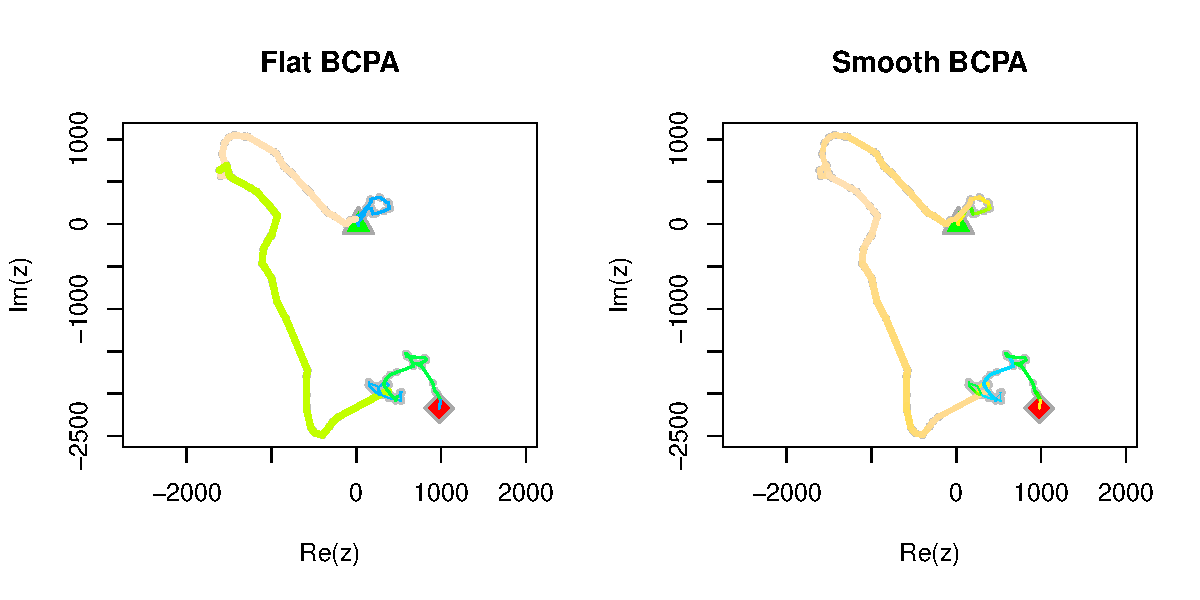
\includegraphics[width=\maxwidth]{figure/BCPApaths} 

\end{knitrout}

The width of the line is proportional to the mean speed, while the colors correspond to the time-scales in the plots above.  Both of thse plots clearly separate the period of faster, more directed movement

An additional, potentially interesting visualization of the analysis is the ``phase plot'', which illustrates how the three parameters change with respect to each other:


\bc
\begin{knitrout}
\definecolor{shadecolor}{rgb}{0.969, 0.969, 0.969}\color{fgcolor}\begin{kframe}
\begin{alltt}
\hlkwd{PhasePlot}\hlstd{(Simp.ws,} \hlkwc{type} \hlstd{=} \hlstr{"smooth"}\hlstd{,} \hlkwc{clusterwidth} \hlstd{=} \hlnum{3}\hlstd{)}
\end{alltt}
\end{kframe}
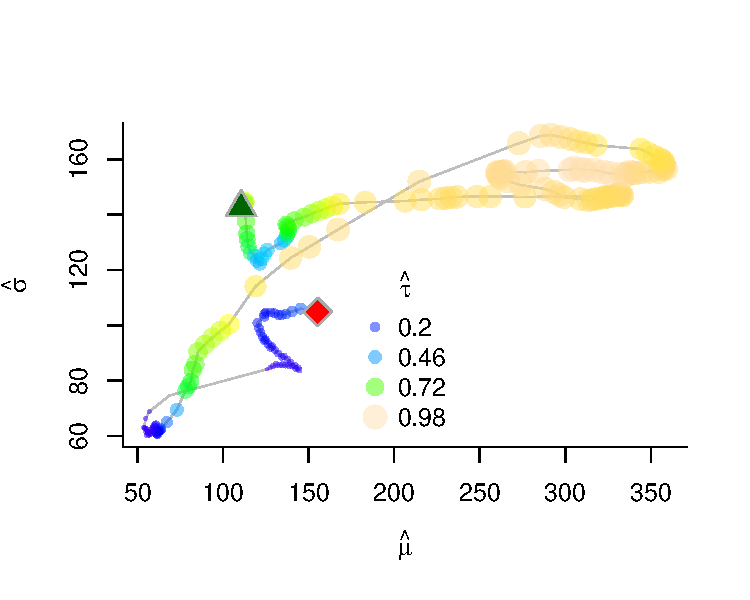
\includegraphics[width=0.6\textwidth]{figure/unnamed-chunk-10} 

\end{knitrout}

\ec

Finally, it is important to assess the assumptions of the BCPA using diagnostic plots. In particular, to assess whether the standardized residuals of the final model are indeed distributed roughly as ${\cal N}(0,1)$ random variables

\bc
\begin{knitrout}
\definecolor{shadecolor}{rgb}{0.969, 0.969, 0.969}\color{fgcolor}\begin{kframe}
\begin{alltt}
\hlkwd{DiagPlot}\hlstd{(Simp.ws)}
\end{alltt}
\end{kframe}
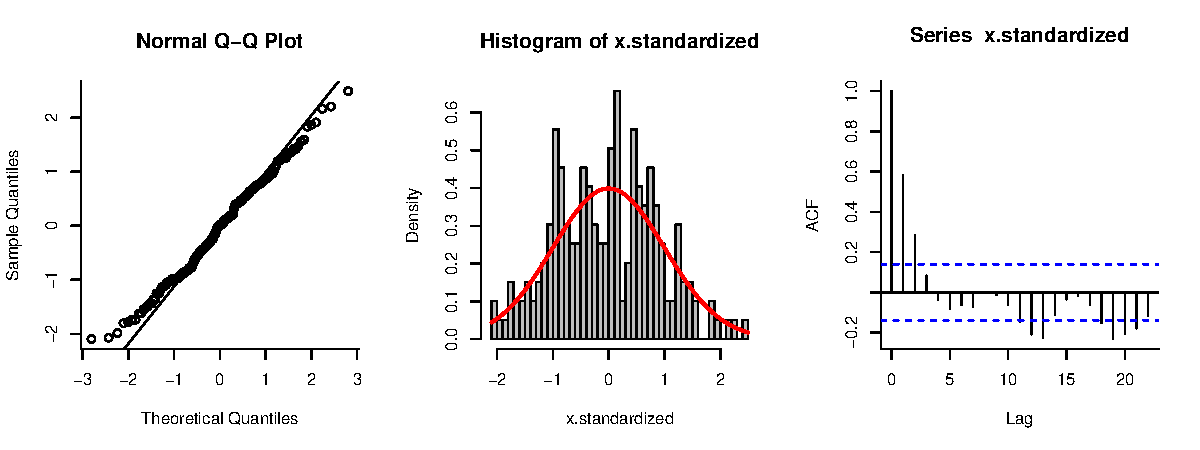
\includegraphics[width=0.8\textwidth]{figure/DiagnosticPlot} 

\end{knitrout}

\ec

This plot illustrates the qq-norm plot, the histogram and the auto-correlation function of the standardized data ($Z_i = X_i - \widehat{\mu}(T_i) / \widehat{\sigma}(T_i)$).  Overall the results seem to satisfy the assumptions of normality. 


\section{Conclusions}

It is hoped that this package will facilitate analysis of complex behavioral movement data.  However, it should be stressed that this is perhaps first and foremost an exploratory tool.  Its strength is that it can distill complex information into some tabulated and visual summaries that outline underlying structures.  It is also relatively fast - a long data set with tens of thousands of locations takes well under a minute to analyze on most machines.  

That said, this tool merely \emph{describes} and does not \emph{explain} complex behavioral profiles.  The BCPA can be used to propose some appropriate movement models or behavioral hypotheses for further testing.  Alternatively, an explanatory or predictive analysis of behaviors with respect to covariates can be performed by extracting some biologically meaningful summary from the BCPA, and performing a post-hoc analysis to model the observed patterns with respect to covariates.   


\section{Acknowledgments}

Gratitude is extended to F.~Cagnacci, M.~Panzacchi, B.~van Moorter and colleagues at the Norwegian Institute of Nature Institute, who organized an animal movement analysis workshop and spearheaded a special issue of J.~Animal Ecology (in progress), lighting the fuse to finally follow through on this package. C.~Bracis and G.~Passolt helped with the technical aspects of finalizing this package.  Thanks, finally, to the many diverse colleagues and animal movement ecologists that tested earlier versions on actual data.  

\section{References}

\begin{description}

\item Gurarie, E., R.~Andrews and K.~Laidre. 2009. A novel method for identifying behavioural changes in animal movement data. Ecology Letters. 12: 395-408.
\item Gurarie, E., O.~Ovaskainen. 2011. Characteristic spatial and temporal scales unify models of animal movement. American Naturalist. 178: 113-123.

\end{description}

\end{document}
